
\begin{wrapfigure}{l}{0cm}
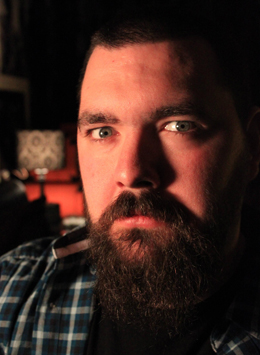
\includegraphics[width=0.3\textwidth]{images/author-main.jpg}
\end{wrapfigure}

Herman R. Huges was born in Bitche, France during the summer of 1966. His
parents, Theodore R. Huges and Gracy W. Huges, were popular folks in their
native town. Herman himself was known as a “troubled child.” He saw many psychologists,
but none could diagnose him. He eventually took to calling his disease “An ailment of
intelligence” and to all observing him this was true. He excelled in school and
did particularly well in his writing courses. His papers while controversial,
were always magnificently written and showcased his unique writing style. A
quote from one of his earlier writings says "The concept of natural coitus is a
strange one. It baffles even the most intelligent minds.". This quote can be
called the defining moment of his life, it laid the foundation for all of his
future work, and the best part is, he wrote it when he was only 15.


       Later in life Herman moved to the U.S. in order to attend the university
of Utah. He eventually got a PhD in gender studies. His professor said this
“Herman was my best and brightest student. He always excelled in my class”. After
graduation Herman went on to work a menial job bagging groceries at a wal-mart.
While there his boss, an extremely radical feminist, constantly berated him and
made his life “a living hell” said Herman. Eventually, not able to take it
anymore, Herman brutally murdered his boss. This landed him a 20 year sentence in
California State Penitentiary. While in prison Herman wrote about his experience,
here is an excerpt from his diary, “The prison system of the U.S. is a barbaric
one. Whatever you do, they don't care. I was raped by 3 men today. They called
it a skullfuck. They put a lock in a sock and bashed my teeth out then proceeded
to force me into performing fellatio.” It may be noted that Herman wears a set
of dentures now.


       Following his release, Herman found solace in writing. None of his
material has been released due to its controversial nature. His most promising
book, though, is currently in the works and is scheduled to be released in late
June or early July. His writing style is very unique, Taking topics that may
seem controversial to some and discussing them on an academic level. He is
considered by some to be “The Next Homer”. His education in his field of writing
may not be magnificent, but he is extremely knowledgeable about the topics
discussed in his books.
